% Cheap Decomposition, Expensive Execution — ACL Workshop Style (two-column)
% Compile: pdflatex main.tex (×2 for references)
\documentclass[11pt,a4paper]{article}

% ─── Two-column ACL-like layout ─────────────────────────────
\usepackage[a4paper,margin=2.5cm,columnsep=0.6cm]{geometry}
\usepackage{multicol}
\usepackage{times}
\usepackage[T1]{fontenc}
\usepackage[utf8]{inputenc}
\usepackage{microtype}
\usepackage{graphicx}
\usepackage{booktabs}
\usepackage{amsmath,amssymb}
\usepackage{xcolor}
\usepackage{hyperref}
\usepackage{natbib}
\usepackage{caption}
\usepackage{enumitem}
\usepackage{float}

% Colors
\definecolor{aclblue}{HTML}{0072B2}
\hypersetup{colorlinks=true,linkcolor=aclblue,citecolor=aclblue,urlcolor=aclblue}

% Compact spacing
\setlength{\parskip}{0pt}
\setlength{\parindent}{1em}
\setlist{nosep,leftmargin=1.2em}
\setlength{\emergencystretch}{3em}
\captionsetup{font=small,labelfont=bf}

% ─── Title block ─────────────────────────────────────────────
\title{\textbf{Cheap Decomposition, Expensive Execution:\\Quantifying the Planning Quality Gap in Multi-Turn Tool-Agent Tasks}}

\author{
  Bo-Yu Chen\\
  \texttt{boyu.chen@my.utsa.edu}
}
\date{}

\begin{document}
\maketitle
\begin{multicols}{2}

% ═══════════════════════════════════════════════════════════════
\section*{Abstract}
% ═══════════════════════════════════════════════════════════════

Multi-turn tool-agent tasks require both planning (what sub-tasks to perform) and execution (how to perform them). We ask: can a lightweight pre-planner improve agent reliability on $\tau$-bench, a customer-service benchmark where state-of-the-art agents fail on over 40\% of tasks? We define \emph{pre-execution planning} as parsing a compound user request into typed sub-goal triples before any tool call, and test five conditions: no planning (baseline), rule-based, automated (Claude Haiku~4.5, \$0.0007/call), same-model (gpt-4o as both planner and executor), and oracle (gold sub-goals). On 22 complex retail tasks across 3 seeds, oracle planning improves mean pass\textsuperscript{1} by 22.7 percentage points (OR=3.5, directionally consistent across all seeds), but both automated planners gain 0--1.5\,pp ($p>0.8$). A same-model ablation rules out model capability as the driver: gpt-4o as decomposer performs identically to Claude Haiku~4.5 ($p=1.0$). A majority-vote robustness check (pass if $\geq$2/3 seeds succeed, $n=22$ independent tasks) confirms the direction of improvement but is underpowered to detect significance ($p=0.75$); we report effect sizes throughout. Pre-execution planning has high headroom when sub-goal quality is sufficient, but automated decomposers, regardless of model size, capture roughly half of the necessary sub-goal structure from the first utterance. We release code and annotations.\footnote{Code: \url{https://github.com/drewOrc/tau-bench-decomposition}}


% ═══════════════════════════════════════════════════════════════
\section{Introduction}
% ═══════════════════════════════════════════════════════════════

Function-calling agents can now handle multi-turn customer-service conversations, but they remain unreliable. On $\tau$-bench \citep{yao2024tau}, a benchmark of realistic retail and airline support tasks with tool use and policy constraints, state-of-the-art agents pass individual tasks at roughly 60\% (pass\textsuperscript{1}) and succeed on the same task three times in a row at only 35\% (pass\textsuperscript{3}). This reliability gap is the central barrier to deployment.

In cost-aware deployment, the question is not ``which model is best?'' but ``where can a cheaper model substitute without quality loss?'' Two substitution points exist. First, a cheap executor with an expensive planner: quality is expected to degrade because execution in multi-turn tool-agent tasks requires policy compliance, error handling, and multi-step API orchestration. Second, a cheap planner with an expensive executor: untested on multi-turn agents. We test the second option.

We propose \emph{pre-execution planning}: before the agent makes any tool call, a lightweight model parses the user request into an ordered sub-goal list. Each sub-goal is a triple of (action\_type, entity, constraint) that specifies what operation to perform, on what object, under what conditions. The agent then executes sub-goals using its full capabilities through the standard function-calling loop.

Our main finding: oracle planning (gold sub-goals) improves pass\textsuperscript{1} by 22.7\,pp (OR=3.5), but automated planners, including a same-model ablation using the executor model itself, gain 0--1.5\,pp. The 22.7\,pp \emph{planning quality gap} is diagnostically interpretable: both automated planners generate half the oracle's sub-goals and cannot resolve entity ambiguity from the first utterance alone. Contributions: (1)~a formal definition of pre-execution planning for multi-turn tool-agent tasks, (2)~a 7-category failure taxonomy of 215 failed trajectories, and (3)~a five-condition experiment isolating the planning ceiling, including a same-model ablation that rules out model capability as the primary driver.


% ═══════════════════════════════════════════════════════════════
\section{Related Work}
% ═══════════════════════════════════════════════════════════════

Two axes organize prior work: \emph{when} decomposition occurs and \emph{whether} the decomposer and executor share the same model.

\paragraph{Upfront decomposition, same model.} Plan-and-Solve \citep{wang2023plan} and Least-to-Most \citep{zhou2023least} decompose problems before solving, in single-turn, tool-free settings. Decomposed Prompting \citep{khot2023decomposed} routes sub-problems to specialized prompts, demonstrating that decomposition and execution need not share the same prompt or model. Our work ports this intuition to multi-turn tool-agent tasks and splits the two stages across models of different cost.

\paragraph{As-needed decomposition, same model.} ReAct \citep{yao2023react} interleaves reasoning with tool actions, forming the default agent loop in $\tau$-bench. ADaPT \citep{prasad2024adapt} recursively decomposes on failure. Tree of Thoughts \citep{yao2023tree} explores reasoning paths with backtracking. Reflexion \citep{shinn2023reflexion} stores verbal self-critiques across attempts. All use the same model for both stages and most incur multiplicative cost. Our decomposer is proactive and costs 0.08\% of the executor.

\paragraph{Cost-aware model selection.} FrugalGPT \citep{chen2023frugalgpt} cascades models for single-turn QA. HuggingGPT \citep{shen2023hugginggpt} routes sub-tasks to specialist \emph{executors}; we use the same executor for all sub-goals with only the \emph{planning} stage delegated. Our earlier work \citep{chen2026routing} applies this principle to single-turn classification; the present paper extends it to multi-turn planning.

\paragraph{$\tau$-bench.} \citet{yao2024tau} introduce $\tau$-bench with pass\textsuperscript{k} exposing brittleness invisible to pass\textsuperscript{1}. No prior work tests upfront decomposition with a cheaper model on a multi-turn tool-agent benchmark.


% ═══════════════════════════════════════════════════════════════
\section{Method}
% ═══════════════════════════════════════════════════════════════

\subsection{Pre-Execution Planning}\label{sec:definition}

We define \emph{pre-execution planning} as parsing a compound user request into an ordered sub-goal list before any tool call. Each sub-goal is a triple of (action\_type, entity, constraint). Action-type specifies which category of operation to perform: in $\tau$-retail, the six types are \textsc{modify}, \textsc{exchange}, \textsc{return}, \textsc{cancel}, \textsc{address}, and \textsc{info}. Entity identification specifies \emph{what} to operate on; the downstream mapping to database IDs is execution. Constraints encode decision rules or are null for unconditional actions.

Unlike Plan-and-Solve \citep{wang2023plan} and Least-to-Most \citep{zhou2023least}, which decompose reasoning problems without specifying operation types, our definition targets proactive, one-shot planning with typed sub-goals. We reserve \emph{execution} for resolving sub-goals into tool calls: database ID discovery, API parameter selection, and policy compliance. Our planning step augments the agent's existing ReAct loop \citep{yao2023react}.

\subsection{Five Planning Conditions}\label{sec:conditions}

\paragraph{Baseline (no planning).} The standard function-calling setup in $\tau$-bench.

\paragraph{Rule-based.} A regex-based decomposer extracts action verbs and entity patterns from the user's first utterance. Cost: \$0. On the full 115-task retail set, 27.5\% of tasks receive zero sub-goals and 61.4\% receive only one.

\paragraph{Oracle.} A human annotator produces gold sub-goal triples from task instructions and ground-truth actions. We construct oracle sub-goals for 22 complex tasks selected by two criteria: $\geq$7 ground-truth actions (top 19\% of action-count distribution) and baseline pass rate below 3/3. This subset selection conditions on baseline performance, so absolute numbers are specific to these 22 tasks; relative comparisons across conditions remain valid.

\paragraph{Automated (tiny-LM).} Claude Haiku~4.5 receives the user's first utterance and a structured prompt requesting JSON sub-goals. Cost: ${\sim}\$0.0007$/call (0.08\% of executor cost).

\paragraph{Same-model (ablation).} gpt-4o as both decomposer and executor, with the identical prompt and output format as the tiny-LM condition. Cost: ${\sim}\$0.001$/call. If the quality gap is model-driven, same-model should approach oracle; if information-limited, it should cluster with tiny-LM.

All five conditions share the same executor (gpt-4o, 2026 snapshot, temperature~0), user simulator (gpt-4o), and seeds (42, 43, 44). The decomposer output is injected into the agent's system prompt at turn~0; all subsequent turns proceed through the standard $\tau$-bench pipeline.


% ═══════════════════════════════════════════════════════════════
\section{Failure Taxonomy}\label{sec:taxonomy}
% ═══════════════════════════════════════════════════════════════

We annotate all 215 failed baseline trajectories (139 retail, 76 airline) using an LLM-as-judge pipeline \citep{zheng2023judging}. A gpt-4o-mini judge classifies each failure into one of seven categories. A 10-sample human spot-check yields 80\% agreement on failure category (8/10). Disagreements arise when the judge labels incomplete execution as \texttt{partial\_resolve} where the human identifies an underlying \texttt{wrong\_decision}. The spot-check identifies one \texttt{user\_led\_astray} case (10\%) where the judge reports 0\%, confirming under-annotation.

\begin{center}
\small
\captionof{table}{Failure taxonomy (LLM-as-judge, $n$=215).}
\label{tab:taxonomy}
\begin{tabular}{lrr}
\toprule
Category & Retail & Airline \\
\midrule
wrong\_decision & 48.2\% & 65.8\% \\
partial\_resolve & 39.6\% & 26.3\% \\
wrong\_argument & 8.6\% & 3.9\% \\
wrong\_info & 2.9\% & 3.9\% \\
user\_led\_astray & 0\% & 0\% \\
unknown & 0.7\% & 0\% \\
\bottomrule
\end{tabular}
\end{center}

Two categories dominate: \texttt{wrong\_decision} and \texttt{partial\_resolve} together account for 87.8\% of retail and 92.1\% of airline failures. We flag one known bias: the decomposition-relevant flag is set at ${\sim}$98\%, likely inflated; the human spot-check suggests ${\sim}$80\%. Our oracle experiment (\S\ref{sec:main}) provides a stronger test of the planning hypothesis than the taxonomy alone.


% ═══════════════════════════════════════════════════════════════
\section{Experiments and Results}\label{sec:experiments}
% ═══════════════════════════════════════════════════════════════

\subsection{Baseline Reproduction}

We reproduce the $\tau$-bench baseline with the 2026 gpt-4o snapshot: $\tau$-retail 59.7\% $\pm$ 10.3\,pp (paper: 61.2\%), $\tau$-airline 49.3\% $\pm$ 4.2\,pp (paper: 35.2\%), 3 seeds. Our retail mean falls within the paper's range; airline is higher, likely reflecting model improvements.

\subsection{Main Results}\label{sec:main}

Table~\ref{tab:main} presents the main experiment on 22 complex retail tasks. The oracle condition improves mean pass\textsuperscript{1} by 22.7\,pp over the baseline (OR=3.5 in pooled analysis; directionally consistent across all three seeds; see \S\ref{sec:stats} for majority-vote robustness analysis). The tiny-LM gains only 1.5\,pp ($p=1.0$). The same-model ablation gains 0.0\,pp ($p=0.838$), ruling out model capability as the primary driver. Oracle pass\textsuperscript{3} reaches 7/22 (31.8\%) vs.\ baseline 0/22 (0\% by selection criterion).

\begin{center}
\small
\captionof{table}{Five-condition comparison (22 complex retail tasks, 3 seeds). $^\dagger$Pooled $n$=66; within-task correlation inflates effective $n$. Majority-vote ($n$=22) yields $p$=0.75; see \S\ref{sec:stats}.}
\label{tab:main}
\setlength{\tabcolsep}{3pt}
\begin{tabular}{@{}lccccc@{}}
\toprule
Condition & S42 & S43 & S44 & Mean$\pm$std & $\Delta$ \\
\midrule
Baseline & 50.0 & 45.5 & 9.1 & 34.8$\pm$22.4 & --- \\
Rule-based & 45.5 & 36.4 & 18.2 & 33.3$\pm$13.9 & $-$1.5 \\
\textbf{Oracle} & \textbf{72.7} & \textbf{54.5} & \textbf{45.5} & \textbf{57.6$\pm$13.9} & \textbf{+22.7}$^\dagger$ \\
Tiny-LM & 31.8 & 36.4 & 40.9 & 36.4$\pm$4.5 & +1.5 \\
Same-model & 36.4 & 36.4 & 31.8 & 34.8$\pm$2.6 & +0.0 \\
\bottomrule
\end{tabular}
\end{center}

The planning quality gap, defined as the difference between oracle and same-model planning, is \textbf{22.7\,pp} (oracle 57.6\% vs.\ same-model 34.8\%; same-model chosen as reference because it controls for model capability). The gap against tiny-LM is 21.2\,pp.

Figure~\ref{fig:conditions} visualises the main result. Oracle planning is the only condition with meaningful improvement; the overlapping error bars between oracle and baseline illustrate why the majority-vote test ($n$=22) lacks power despite a large effect size.

\begin{center}
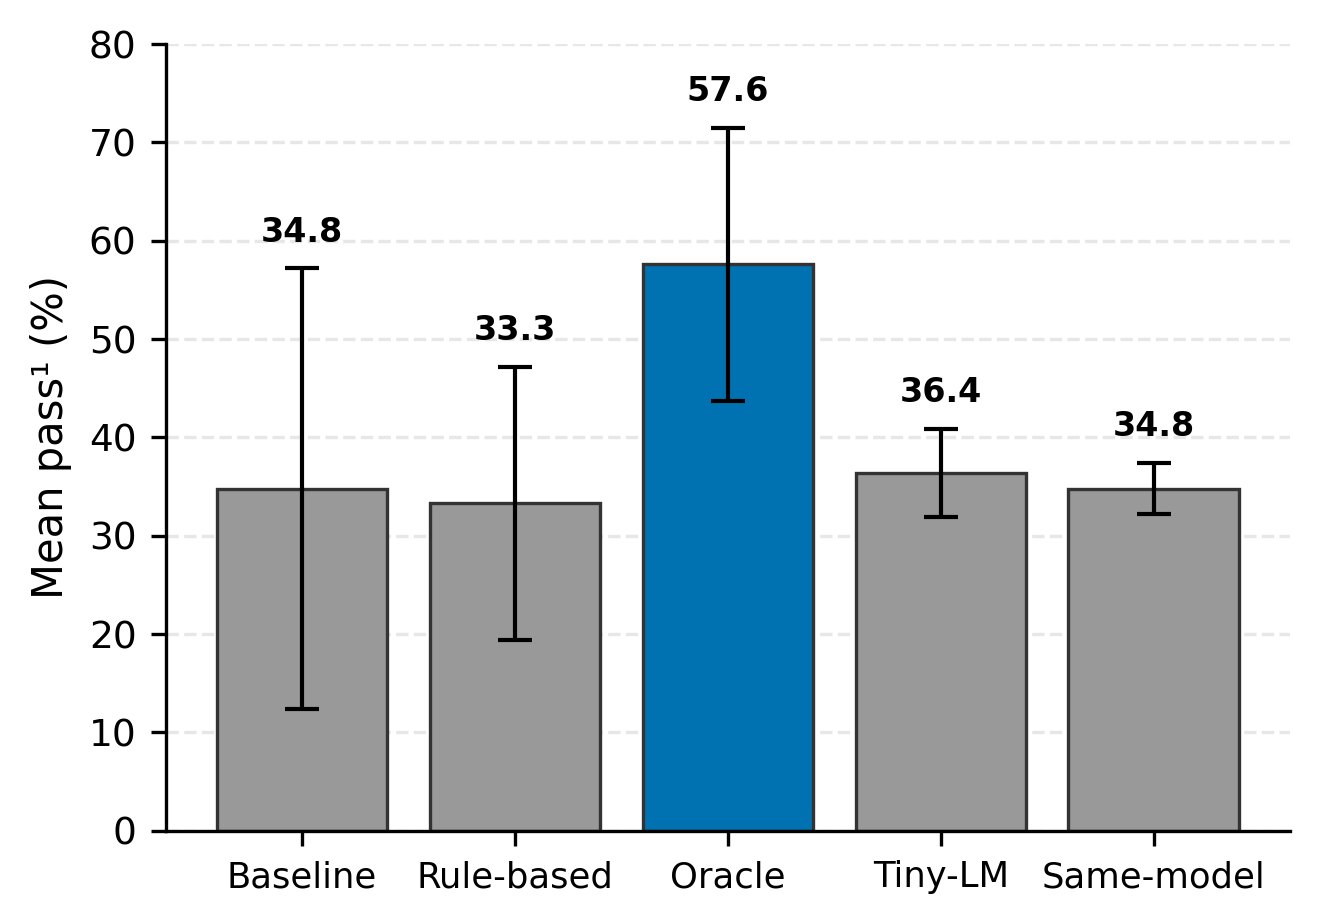
\includegraphics[width=\linewidth]{figures/fig_conditions.png}
\captionof{figure}{Mean pass$^1$ ($\pm$1 std across 3 seeds) for five planning conditions on 22 complex retail tasks. Oracle planning (+22.7\,pp) is the only condition with meaningful improvement. Automated planners also reduce cross-seed variance (narrowing error bars).}
\label{fig:conditions}
\end{center}


\subsection{Statistical Tests}\label{sec:stats}

We use McNemar's test with continuity correction on paired binary outcomes (22 tasks $\times$ 3 seeds = 66 pooled observations).

The oracle shows asymmetric improvement in pooled analysis ($n$=66): 21 tasks flip fail-to-pass vs.\ 6 pass-to-fail (OR=3.5, $p$=0.007). Same-model vs.\ baseline: $b$=12, $c$=12, $p$=0.838, OR=1.0. Same-model vs.\ tiny-LM: $p$=1.0. Holm--Bonferroni correction: oracle vs.\ baseline survives ($\alpha$/6=0.0083); oracle vs.\ tiny-LM ($p$=0.018) does not ($\alpha$/5=0.010). Direction is consistent across all three seeds (net discordant: +5, +2, +8).

\textbf{Independence caveat.} Pooling treats 66 pairs as independent, but within-task outcomes share task instructions across seeds. A leave-one-seed-out analysis: without seed~44, $p$=0.146; the other two remain significant.

\textbf{Majority-vote robustness.} Aggregating per-task (pass if $\geq$2/3 seeds succeed) yields $n$=22 independent observations. Oracle 50.0\% vs.\ baseline 40.9\%, +9.1\,pp, $p$=0.75. The loss of significance reflects reduced power (10 vs.\ 27 discordant pairs), not a reversal: oracle maintains the highest majority-vote rate across all five conditions. We report effect sizes as primary evidence throughout.


\subsection{Variance Stabilization}

All planning conditions reduce cross-seed variance. The coefficient of variation drops monotonically: baseline 0.64, rule-based 0.42, oracle 0.24, tiny-LM 0.12, same-model 0.08 (an $8\times$ reduction). The same-model planner achieves the lowest CV despite no accuracy gain, suggesting that structural pre-planning stabilizes agent behavior even when sub-goal quality is low.


\subsection{Diagnosing the Quality Gap}

Why does automated planning fail to capture oracle-level quality? Table~\ref{tab:quality} compares sub-goal characteristics.

\begin{center}
\small
\captionof{table}{Sub-goal quality comparison.}
\label{tab:quality}
\setlength{\tabcolsep}{4pt}
\begin{tabular}{@{}lccc@{}}
\toprule
Metric & Oracle & Tiny-LM & Same \\
\midrule
Mean sub-goals/task & 3.0 & 1.5 & 1.4 \\
Distinct action types & 6 & 1.4 & 6 \\
Entities ``(unclear)'' & 0\% & 18\% & 30\% \\
Tasks $<$0.5$\times$ oracle & 0/22 & 10/22 & 15/22 \\
\bottomrule
\end{tabular}
\end{center}

The primary failure mode is \emph{under-decomposition}: both automated planners generate $<$50\% of oracle sub-goals (1.5 and 1.4 vs.\ 3.0). The same-model planner uses all 6 action types but still under-decomposes and marks 30\% of entities as ``(unclear).'' For example, Task~23 requires three operations (exchange helmet, exchange luggage set, modify grill). Both automated planners produce a single sub-goal targeting only the helmet. The identical failure pattern despite gpt-4o costing 1.4$\times$ more per call rules out model capability as the primary driver; the bottleneck is information available in the first utterance.

Both decomposers add $<$0.12\% of executor cost (\$0.0007--\$0.001/call vs.\ ${\sim}$\$0.85/task). The bottleneck is decomposition \emph{quality}, not cost.


% ═══════════════════════════════════════════════════════════════
\section{Discussion}
% ═══════════════════════════════════════════════════════════════

\subsection{When Does Cheap-Plan-Expensive-Execute Work?}

Oracle planning yields the largest gain (+22.7\,pp, OR=3.5). Neither automated condition improves: the same-model ablation (+0.0\,pp, discordant pairs 12:12) rules out model capability, since even the executor model cannot produce useful decompositions from the first utterance alone. All planning conditions reduce cross-seed variance (baseline CV=0.64 $\to$ same-model CV=0.08), suggesting that structural pre-planning stabilizes behavior even when sub-goal quality is low.

\subsection{The Quality Gap as a Research Target}

The 22.7\,pp gap quantifies the improvement available if decomposer quality can be raised. Three shared failure modes suggest directions:

\begin{enumerate}
\item \textbf{Under-decomposition.} Mean 1.5 sub-goals vs.\ oracle's 3.0; 45--68\% of tasks receive $<$50\% of oracle sub-goals.
\item \textbf{Action-type collapse.} The tiny-LM planner defaults to 1--2 action types (mean 1.4) vs.\ oracle's full range of 6; the same-model planner uses all 6 types but still under-decomposes.
\item \textbf{Entity ambiguity.} 18--30\% of entities marked unclear. The first utterance uses pronouns and partial descriptions.
\end{enumerate}

Multi-turn context, retrieval-augmented planning, or domain-specific schemas could address these.

\subsection{Limitations}

\begin{enumerate}
\item \textbf{Single benchmark.} Generalization to WebArena \citep{zhou2024webarena} or SWE-bench \citep{jimenez2024swebench} is untested.
\item \textbf{Single executor.} Weaker executors may benefit more; stronger executors (o1-class) may benefit less.
\item \textbf{No human-human IAA.} The LLM-as-judge has known biases; an 80\% human-LLM spot-check (\S\ref{sec:taxonomy}) provides partial validation.
\item \textbf{Small task subset.} Majority-vote robustness ($n$=22) confirms direction but lacks power ($p$=0.75); the oracle effect should be interpreted through effect size (OR=3.5) and cross-seed consistency.
\item \textbf{Single oracle annotator} with access to ground-truth actions. A second annotator would strengthen validity.
\end{enumerate}


% ═══════════════════════════════════════════════════════════════
\section{Conclusion}
% ═══════════════════════════════════════════════════════════════

On $\tau$-bench compound tasks, pre-execution planning has high headroom: oracle sub-goals improve pass\textsuperscript{1} by 22.7\,pp (OR=3.5, directionally consistent) and achieve pass\textsuperscript{3} of 31.8\% (vs.\ 0\% by selection criterion). A majority-vote robustness check ($n$=22) confirms the direction but is underpowered; the evidence rests on effect size and cross-seed consistency. Neither automated planner (Claude Haiku~4.5 nor gpt-4o) yields significant gain. The same-model ablation is our most precise finding: model capability alone does not close the 22.7\,pp quality gap ($p$=1.0), suggesting the first utterance lacks sufficient information.

The decomposer adds $<$0.12\% of executor cost. Cost is not the bottleneck; decomposition quality is. Closing the gap requires decomposers that operate on more than the first utterance: multi-turn context, retrieval-augmented planning, or domain-specific schemas. We release all code, oracle sub-goals, and failure annotations.

% ═══════════════════════════════════════════════════════════════
\section*{Acknowledgments}
% ═══════════════════════════════════════════════════════════════

We thank the $\tau$-bench authors for releasing their benchmark and code. An LLM assistant (Claude, Anthropic) was used for proofreading and stylistic editing of the manuscript. All research design, experiments, analysis, and initial drafting were conducted solely by the author.

% ═══════════════════════════════════════════════════════════════
\section*{Reproducibility Statement}
% ═══════════════════════════════════════════════════════════════

Code, oracle sub-goals, failure annotations, and per-seed trajectories: \url{https://github.com/drewOrc/tau-bench-decomposition} (MIT). Executor and user simulator: gpt-4o (2026 snapshot, temperature~0). Decomposer (tiny-LM): \texttt{claude-haiku-4-5-20251001}. Same-model decomposer: gpt-4o with identical prompt. Seeds: 42, 43, 44. Executor cost: ${\sim}$\$0.85/task. The five-condition experiment runs 22 tasks $\times$ 3 seeds $\times$ 5 conditions; baseline reproduction runs 165 tasks $\times$ 3 seeds. Total experiment cost: approximately \$180.

% ═══════════════════════════════════════════════════════════════
% References
% ═══════════════════════════════════════════════════════════════

\begin{thebibliography}{14}

\bibitem[Chen(2026)]{chen2026routing}
Bo-Yu Chen. 2026.
\newblock Cost-Aware Hybrid Routing for Intent Classification: 74\% {LLM} Cost Reduction at Equal Accuracy.
\newblock \emph{arXiv preprint}.

\bibitem[Chen et~al.(2023)]{chen2023frugalgpt}
Lingjiao Chen, Matei Zaharia, and James Zou. 2023.
\newblock {FrugalGPT}: How to Use Large Language Models While Reducing Cost and Improving Performance.
\newblock In \emph{Proceedings of ICML}.

\bibitem[Jimenez et~al.(2024)]{jimenez2024swebench}
Carlos~E. Jimenez, John Yang, Alexander Wettig, Shunyu Yao, Kexin Pei, Ofir Press, and Karthik Narasimhan. 2024.
\newblock {SWE}-bench: Can Language Models Resolve Real-World {GitHub} Issues?
\newblock In \emph{Proceedings of ICLR}.

\bibitem[Khot et~al.(2023)]{khot2023decomposed}
Tushar Khot, Harsh Trivedi, Matthew Finlayson, Yao Fu, Kyle Richardson, Peter Clark, and Ashish Sabharwal. 2023.
\newblock Decomposed Prompting: A Modular Approach for Solving Complex Tasks.
\newblock In \emph{Proceedings of ICLR}.

\bibitem[Prasad et~al.(2024)]{prasad2024adapt}
Archiki Prasad, Alexander Koller, Mareike Hartmann, Peter Clark, Ashish Sabharwal, Mohit Bansal, and Tushar Khot. 2024.
\newblock {ADaPT}: As-Needed Decomposition and Planning with Language Models.
\newblock In \emph{Proceedings of NAACL}.

\bibitem[Shen et~al.(2023)]{shen2023hugginggpt}
Yongliang Shen, Kaitao Song, Xu Tan, Dongsheng Li, Weiming Lu, and Yueting Zhuang. 2023.
\newblock {HuggingGPT}: Solving {AI} Tasks with {ChatGPT} and its Friends in {Hugging Face}.
\newblock In \emph{Proceedings of NeurIPS}.

\bibitem[Shinn et~al.(2023)]{shinn2023reflexion}
Noah Shinn, Federico Cassano, Ashwin Gopinath, Karthik Narasimhan, and Shunyu Yao. 2023.
\newblock Reflexion: Language Agents with Verbal Reinforcement Learning.
\newblock In \emph{Proceedings of NeurIPS}.

\bibitem[Wang et~al.(2023)]{wang2023plan}
Lei Wang, Wanyu Xu, Yihuai Lan, Zhiqiang Hu, Yunshi Lan, Roy Ka-Wei Lee, and Ee-Peng Lim. 2023.
\newblock Plan-and-Solve Prompting: Improving Zero-Shot Chain-of-Thought Reasoning by Large Language Models.
\newblock In \emph{Proceedings of ACL}.

\bibitem[Yao et~al.(2023a)]{yao2023react}
Shunyu Yao, Jeffrey Zhao, Dian Yu, Nan Du, Izhak Shafran, Karthik Narasimhan, and Yuan Cao. 2023a.
\newblock {ReAct}: Synergizing Reasoning and Acting in Language Models.
\newblock In \emph{Proceedings of ICLR}.

\bibitem[Yao et~al.(2023b)]{yao2023tree}
Shunyu Yao, Dian Yu, Jeffrey Zhao, Izhak Shafran, Thomas~L. Griffiths, Yuan Cao, and Karthik Narasimhan. 2023b.
\newblock Tree of Thoughts: Deliberate Problem Solving with Large Language Models.
\newblock In \emph{Proceedings of NeurIPS}.

\bibitem[Yao et~al.(2024)]{yao2024tau}
Shunyu Yao, Ankit Shinde, Karthik Narasimhan, and Yuntao Bai. 2024.
\newblock $\tau$-bench: A Benchmark for Tool-Agent-User Interaction in Real-World Domains.
\newblock \emph{arXiv preprint arXiv:2406.12045}.

\bibitem[Zheng et~al.(2023)]{zheng2023judging}
Lianmin Zheng, Wei-Lin Chiang, Ying Sheng, Siyuan Zhuang, Zhanghao Wu, Yonghao Zhuang, Zi Lin, Zhuohan Li, Dacheng Li, Eric~P. Xing, et~al. 2023.
\newblock Judging {LLM}-as-a-Judge with {MT}-Bench and Chatbot Arena.
\newblock In \emph{Proceedings of NeurIPS}.

\bibitem[Zhou et~al.(2023)]{zhou2023least}
Denny Zhou, Nathaniel Sch{\"a}rli, Le Hou, Jason Wei, Nathan Scales, Xuezhi Wang, Dale Schuurmans, Claire Cui, Olivier Bousquet, Quoc Le, and Ed Chi. 2023.
\newblock Least-to-Most Prompting Enables Complex Reasoning in Large Language Models.
\newblock In \emph{Proceedings of ICLR}.

\bibitem[Zhou et~al.(2024)]{zhou2024webarena}
Shuyan Zhou, Frank~F. Xu, Hao Zhu, Xuhui Zhou, Robert Lo, Abishek Sridhar, Xianyi Cheng, Tianyue Ou, Yonatan Bisk, Daniel Fried, Uri Alon, and Graham Neubig. 2024.
\newblock {WebArena}: A Realistic Web Environment for Building Autonomous Agents.
\newblock In \emph{Proceedings of ICLR}.

\end{thebibliography}

\end{multicols}
\end{document}
